% !TeX root = ../main.tex

\section{RQ3: Component Complexity Analysis}
\vspace{-3pt}

\subsection{Methodology}

To answer \textbf{RQ3}, we classified categories of code snippets in each component and explored their composition patterns. %We collected and analysed quantitative data in the following steps: 
% \todo{Add a code example to show different code cateogries}.

\textbf{Step 1: Label code snippets.} We segmented each source code file into code snippets according to semantic meaning, and then classified them into 6 categories: (1) model definition, the definition code of ML models; (2) rule definition, the definition code of rules in rule-based components; (3) model usage, the usage code of ML models; (4) rule usage, the usage code of rules; (5) data pre-processing, the input data processing code before model or rule usages; (6) data post-processing, the output data processing code after model or rule usages. Two of the authors labeled code snippets independently, and the third author was involved to resolve disagreements. The Cohen's Kappa coefficient of the two authors reached 0.830.
% \todo{add detail labelled example.}

\textbf{Step 2: Summarize composition patterns of code snippets.} 
Based on labeled code snippets, we summarized the composition patterns of data processing code, and model or rule usage code in each component.  

\subsection{Results}
\begin{table}[!t]
	\caption{LoC of Different Code Categories}
	\vspace{-10pt}
    \footnotesize
	\begin{center}
    \tabcolsep=1.0mm
	\begin{tabular}{ccccccc}
        \hline
        \multirow{2}{*}{\textbf{Module}} & \multicolumn{2}{c}{\textbf{Data}} & \multicolumn{2}{c}{\textbf{Model}} & \multicolumn{2}{c}{\textbf{Rule}} \\ \cline{2-7} 
                                              & Pre. & Post.                 & Usage & Definition                  & Usage & Definition \\ \hline
        \multicolumn{1}{c|}{Tokenizer}        &8      & \multicolumn{1}{c|}{80} &27       & \multicolumn{1}{c|}{0} &25       &25      \\
        \multicolumn{1}{c|}{Featurizer}       &390      & \multicolumn{1}{c|}{323} &92       & \multicolumn{1}{c|}{0} &162       &119      \\
        \multicolumn{1}{c|}{IntentClassifier} &441      & \multicolumn{1}{c|}{131} &113       & \multicolumn{1}{c|}{298} &3       &69      \\
        \multicolumn{1}{c|}{EntityExtractor}  &746      & \multicolumn{1}{c|}{311} &120       & \multicolumn{1}{c|}{298} &24       &30      \\
        \multicolumn{1}{c|}{Selector}         &48      & \multicolumn{1}{c|}{55} &9       & \multicolumn{1}{c|}{16} &0       &0      \\
        \multicolumn{1}{c|}{Policy}           &1332     & \multicolumn{1}{c|}{540} &64       & \multicolumn{1}{c|}{543} &167       &283      \\
        \multicolumn{1}{c|}{Shared}           &996      & \multicolumn{1}{c|}{314} &112       & \multicolumn{1}{c|}{1673} &0       &43      \\
        \multicolumn{1}{c|}{Total}            &3961      & \multicolumn{1}{c|}{1754} &537       & \multicolumn{1}{c|}{2828} &381       &569      \\ \hline
        \end{tabular}
	\label{code_type_stat}
	\end{center}
\end{table}

The statistics of different code categories are shown in Table \ref{code_type_stat}. We only considered the LoC of labeled code snippets, while ignoring general utils code such as class initialization. 
Data processing code contributes a total of 5715 (57.1\%) LoC, while model usage\&definition code and rule usage\&definition code contribute 3365 (33.5\%) and 950 (9.4\%) LoC, respectively. 
1673 (59.2\%) of the 2828 LoC of model definition code is in  \textit{Shared} module, which shows that the reuse of model definition code between different components is quite common. There is no model definition code in \textit{Tokenizer} and \textit{Featurizer}, because ML components are all built on top of external ML libraries.

% \todo{a Featurizer has the less propertion of data processing code.} 

We classified data pre-processing and data post-processing categories into more specific types, due to the dominant proportion of data processing code in Rasa. 
Specifically, \textit{Validation} code intends to validate the input or output data of components. \textit{Format Transformation} code transforms data format, such as constructing vectors from Python arrays and reshaping vectors. 
% ensembling data, into a \texttt{Message} class instance for data transmission between components. 
\textit{Component Input/Output Filter} code filters data that does not meet the specified criteria, such as the absence of certain attributes. 
\textit{Data Scale/Padding/Encoding/Decoding} code changes the value of data, while \textit{Data Split/Shuffle/Balance/Batch/Rank} code changes the organization of data for better training and inference of components.
We provide the complete codebook and statistics of data processing types at our website \cite{website}.

\begin{figure*}[ht]
    \centering
    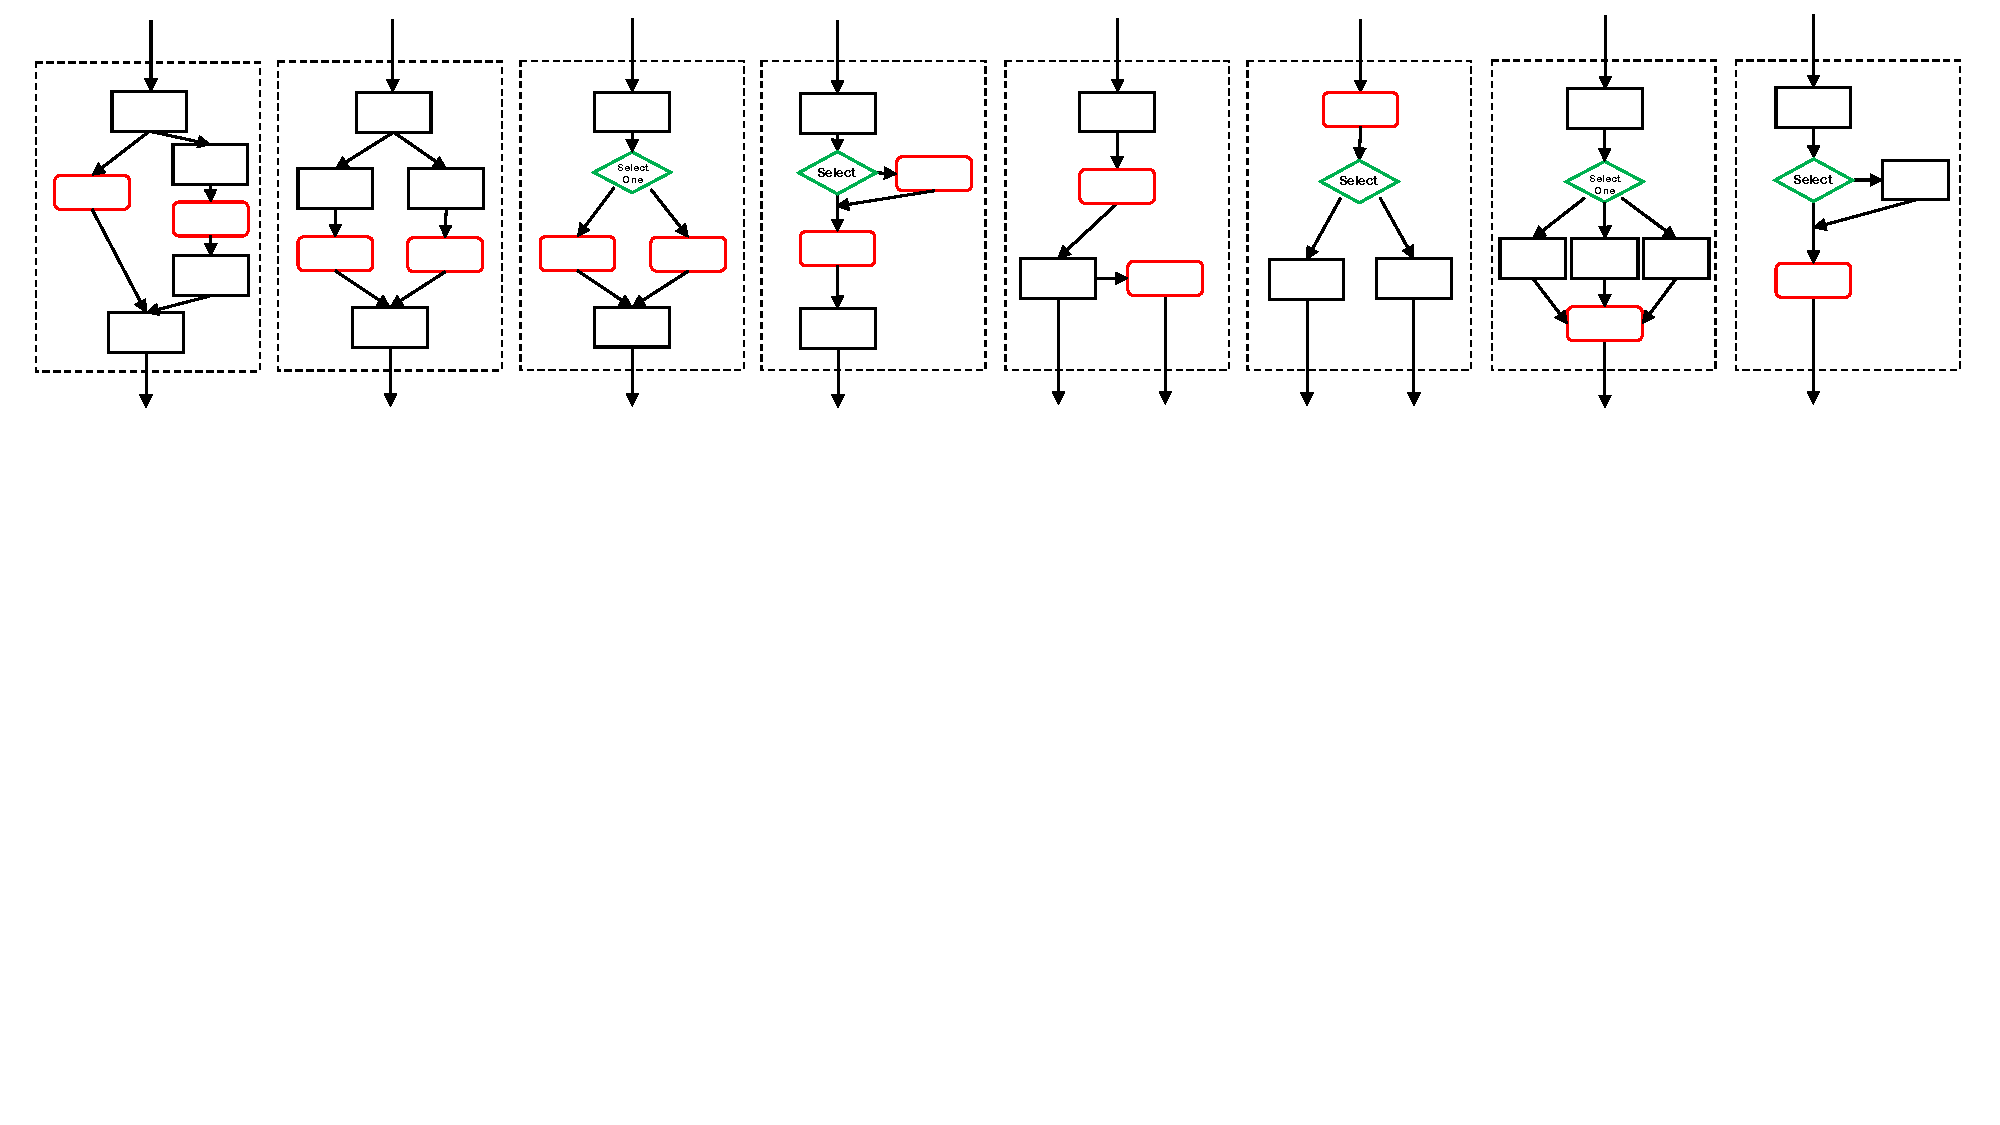
\includegraphics[scale=0.53]{figs/code_composition.pdf}
    \vspace{-10pt}
    \caption{Non-Sequential Code Composition Patterns within Components}
    \label{code_composition}
\end{figure*}

Moreover, we find that composition patterns of code snippets include sequential code composition pattern and various non-sequential composition patterns.
In a typical sequential composition pattern, data is first pre-processed, and then processed by model or rule usage code, and finally post-processed.
The non-sequential code composition patterns are summarized in Fig. \ref{code_composition}. The black box is a data processing code snippet, the red box is a model or rule usage code snippet, and the green diamond means to select one or multiple downstream code snippets.
The first 5 patterns consist of multiple model or rule usages in one component. %, e.g., \textit{ConveRTFeaturizer} component generates sequence and sentence features with two model or rule usages. 
The last 3 patterns consist of a single model or rule usage with multiple possible data processing snippets, decided by configurations or input data.


% \todo{website: add propertion of different code types(data processing code, model usage) in each path.}
% \todo{website: add box figure, for every module, show its Path Num, Pre Num, Pre Line, Post Num, Post Line. For train and predict path, show path num.. (process\_training data). add statistics of different types of code}
% \todo{website: data processing detail type}

\subsection{Implications}
%Our results reflect that the component complexity are from the following aspects.

\textbf{Data processing.} Data processing code is scattered~at~different granularity levels, unlike the well-documented~and~structured code of ML models and rules. 
In detail, data processing code includes data processing components (e.g., \textit{PolicyEnsemble}), general data processing classes and functions in \textit{Shared} module, and specific data processing snippets in components entangled with model or rule usages. 
On the one hand, it could become troublesome for application developers to identify and understand the semantics of all data processing code. A specific example is that data pre-processing code also exists in model definition class of \texttt{TransformerRasaModel}, including \textit{Formant Conversion} and \textit{Data Batch} code. It could be explicitly helpful to automatically extract and analyze the semantics of data processing code  with techniques like program analysis \cite{pycg}. On the other hand, it would be challenging for system developers to maintain and test data processing code, possibly resulting in severe consequences with ML development paradigm shift from model-centric  to data-centric \cite{liangAdvancesChallengesOpportunities2022}. 
In general, building a taxonomy of data processing code would be helpful for maintaining and testing of data processing code.
% the test oracle of data processing code is hard.


\textbf{Code composition patterns.} These non-sequential composition patterns could introduce additional dynamic complexity for ML-enabled systems, e.g., it is too expensive to capture all possible run-time compositions of code snippets~with~static analysis. Although dynamic testing is widely adopted~to~complement the limitations of static analysis in traditional software \cite{fairley1978tutorial}, most existing testing techniques tailored for ML only target the ML model level \cite{ml_testing}. It would be beneficial to extend them to include data processing code and composition patterns.
